\section{Retrieval Augmented Generation (RAG)}
Modelin önceden toplanmış bir bilgi havuzundan yararlanarak daha bilgi odaklı çıktılar üretmesini sağlar. RAG, bir dil modeli ve bir bilgi getirme sisteminden oluşur. Bilgi getirme sistemi bir arama motoru veya bilgi tabanıdır ve bu bilgi tabanından ilgili içeriği getirmek için kullanılır. Yeniden model eğitmeye gerek olmadığı için uygun maliyetli bir yaklaşımdır. Kendi içerisinde 4 gruba ayrılmıştır:

\begin{figure}[h]
    \centering
    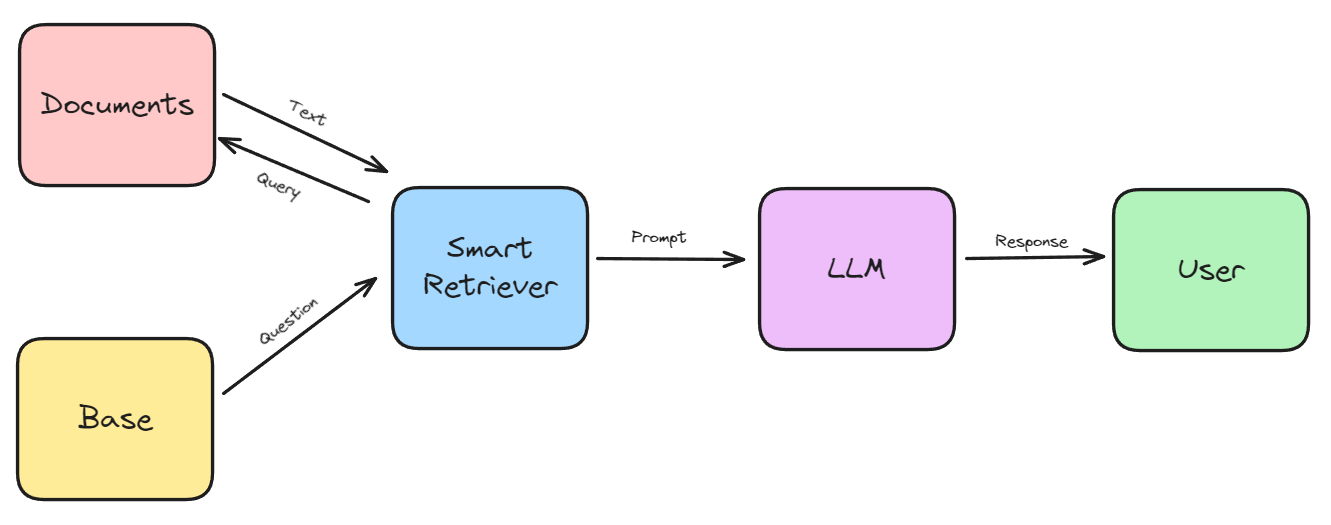
\includegraphics[width=1\textwidth]{images/rag_architecture.png}
    \caption{RAG adımları.}
    \label{fig:enter-label}
\end{figure}

\subsection{Before Generation}
"LLM-Augmenter" ve "FreshPrompt" bu gruba örnektir. FreshPrompt, LLM'e her seferinde farklı bir komut sağlayarak çalışır. Bu komutlar, LLM'in daha önce ürettiği metinlere dayanarak oluşturulabilir. LLM-Augmenter, LLM'in çıktısını üç farklı modül kullanarak analiz eder.
\begin{itemize}
    \item \textbf{Prompt Motoru:} LLM'e sorulacak komutu oluşturur.
    \item \textbf{Fayda Modülü:} LLM'in ürettiği metnin faydasını ve doğruluğunu değerlendirir.
    \item \textbf{Politika Modülü:} LLM'e ne yapması gerektiğini söyler. Örneğin LLM'den daha fazla bilgi istemesi, farklı bir metin üretmesi gibi.
\end{itemize}

\subsection{During Generation}
"Knowledge Retrieval", "Decompose and Query Framework" ve "Real-time Verification and Rectification" bu gruba örnektir. Knowledge Retrieval, üretilen metni bir bilgi kaynağıyla karşılaştırarak çalışır. Tutarsızlık veya yanlış bilgi tespit edilirse, bu bilgileri düzeltir. Decompose and Query Framework (D\&Q), karmaşık bir komutu daha küçük parçalara ayrıştırır. Her parça, ayrı ayrı bir bilgi kaynağında sorgulanır. Her parçadan gelen cevaplar birleştirilerek tek bir cevap oluşturulur. EVER, üretilen metni bir bilgi kaynağı ile karşılaştırır. Tutarsızlık varsa sistem bir hata mesajı üretir. Sistem, hataları otomatik olarak düzeltmeye çalışır veya kullanıcıdan düzeltme için geri bildirim ister.

\subsection{After Generation}
"Retrofit Attribution using Research and Revision" bu gruba örnektir. Retrofit Attribution using Research and Revision üretilen metni bir bilgi kaynağı ile karşılaştırır. Her bilgi parçası için uygun kaynak bulunur. Kaynaklar metne atıf olarak eklenir. Kullanıcı tutarsızlıkları düzeltir.

\subsection{End-to-End RAG}
Önceden eğitilmiş bir Seq2Seq transformer'in Dense Passage Retriever (DPR) üzerinden erişilen Wikipedia'nın vektör dizini ile entegrasyonunu içerir. Bu entegrasyon modelin çıktı üretimini hem girdi sorgusu hem de DPR tarafından sağlanan gizli belgeler üzerinden koşullandırılmasını sağlar.

\newpage